% Options for packages loaded elsewhere
\PassOptionsToPackage{unicode}{hyperref}
\PassOptionsToPackage{hyphens}{url}
\PassOptionsToPackage{dvipsnames,svgnames,x11names}{xcolor}
%
\documentclass[
  letterpaper,
  DIV=11,
  numbers=noendperiod]{scrartcl}

\usepackage{amsmath,amssymb}
\usepackage{iftex}
\ifPDFTeX
  \usepackage[T1]{fontenc}
  \usepackage[utf8]{inputenc}
  \usepackage{textcomp} % provide euro and other symbols
\else % if luatex or xetex
  \usepackage{unicode-math}
  \defaultfontfeatures{Scale=MatchLowercase}
  \defaultfontfeatures[\rmfamily]{Ligatures=TeX,Scale=1}
\fi
\usepackage{lmodern}
\ifPDFTeX\else  
    % xetex/luatex font selection
\fi
% Use upquote if available, for straight quotes in verbatim environments
\IfFileExists{upquote.sty}{\usepackage{upquote}}{}
\IfFileExists{microtype.sty}{% use microtype if available
  \usepackage[]{microtype}
  \UseMicrotypeSet[protrusion]{basicmath} % disable protrusion for tt fonts
}{}
\makeatletter
\@ifundefined{KOMAClassName}{% if non-KOMA class
  \IfFileExists{parskip.sty}{%
    \usepackage{parskip}
  }{% else
    \setlength{\parindent}{0pt}
    \setlength{\parskip}{6pt plus 2pt minus 1pt}}
}{% if KOMA class
  \KOMAoptions{parskip=half}}
\makeatother
\usepackage{xcolor}
\setlength{\emergencystretch}{3em} % prevent overfull lines
\setcounter{secnumdepth}{-\maxdimen} % remove section numbering
% Make \paragraph and \subparagraph free-standing
\makeatletter
\ifx\paragraph\undefined\else
  \let\oldparagraph\paragraph
  \renewcommand{\paragraph}{
    \@ifstar
      \xxxParagraphStar
      \xxxParagraphNoStar
  }
  \newcommand{\xxxParagraphStar}[1]{\oldparagraph*{#1}\mbox{}}
  \newcommand{\xxxParagraphNoStar}[1]{\oldparagraph{#1}\mbox{}}
\fi
\ifx\subparagraph\undefined\else
  \let\oldsubparagraph\subparagraph
  \renewcommand{\subparagraph}{
    \@ifstar
      \xxxSubParagraphStar
      \xxxSubParagraphNoStar
  }
  \newcommand{\xxxSubParagraphStar}[1]{\oldsubparagraph*{#1}\mbox{}}
  \newcommand{\xxxSubParagraphNoStar}[1]{\oldsubparagraph{#1}\mbox{}}
\fi
\makeatother


\providecommand{\tightlist}{%
  \setlength{\itemsep}{0pt}\setlength{\parskip}{0pt}}\usepackage{longtable,booktabs,array}
\usepackage{calc} % for calculating minipage widths
% Correct order of tables after \paragraph or \subparagraph
\usepackage{etoolbox}
\makeatletter
\patchcmd\longtable{\par}{\if@noskipsec\mbox{}\fi\par}{}{}
\makeatother
% Allow footnotes in longtable head/foot
\IfFileExists{footnotehyper.sty}{\usepackage{footnotehyper}}{\usepackage{footnote}}
\makesavenoteenv{longtable}
\usepackage{graphicx}
\makeatletter
\def\maxwidth{\ifdim\Gin@nat@width>\linewidth\linewidth\else\Gin@nat@width\fi}
\def\maxheight{\ifdim\Gin@nat@height>\textheight\textheight\else\Gin@nat@height\fi}
\makeatother
% Scale images if necessary, so that they will not overflow the page
% margins by default, and it is still possible to overwrite the defaults
% using explicit options in \includegraphics[width, height, ...]{}
\setkeys{Gin}{width=\maxwidth,height=\maxheight,keepaspectratio}
% Set default figure placement to htbp
\makeatletter
\def\fps@figure{htbp}
\makeatother
% definitions for citeproc citations
\NewDocumentCommand\citeproctext{}{}
\NewDocumentCommand\citeproc{mm}{%
  \begingroup\def\citeproctext{#2}\cite{#1}\endgroup}
\makeatletter
 % allow citations to break across lines
 \let\@cite@ofmt\@firstofone
 % avoid brackets around text for \cite:
 \def\@biblabel#1{}
 \def\@cite#1#2{{#1\if@tempswa , #2\fi}}
\makeatother
\newlength{\cslhangindent}
\setlength{\cslhangindent}{1.5em}
\newlength{\csllabelwidth}
\setlength{\csllabelwidth}{3em}
\newenvironment{CSLReferences}[2] % #1 hanging-indent, #2 entry-spacing
 {\begin{list}{}{%
  \setlength{\itemindent}{0pt}
  \setlength{\leftmargin}{0pt}
  \setlength{\parsep}{0pt}
  % turn on hanging indent if param 1 is 1
  \ifodd #1
   \setlength{\leftmargin}{\cslhangindent}
   \setlength{\itemindent}{-1\cslhangindent}
  \fi
  % set entry spacing
  \setlength{\itemsep}{#2\baselineskip}}}
 {\end{list}}
\usepackage{calc}
\newcommand{\CSLBlock}[1]{\hfill\break\parbox[t]{\linewidth}{\strut\ignorespaces#1\strut}}
\newcommand{\CSLLeftMargin}[1]{\parbox[t]{\csllabelwidth}{\strut#1\strut}}
\newcommand{\CSLRightInline}[1]{\parbox[t]{\linewidth - \csllabelwidth}{\strut#1\strut}}
\newcommand{\CSLIndent}[1]{\hspace{\cslhangindent}#1}

\KOMAoption{captions}{tableheading}
\makeatletter
\@ifpackageloaded{caption}{}{\usepackage{caption}}
\AtBeginDocument{%
\ifdefined\contentsname
  \renewcommand*\contentsname{Table of contents}
\else
  \newcommand\contentsname{Table of contents}
\fi
\ifdefined\listfigurename
  \renewcommand*\listfigurename{List of Figures}
\else
  \newcommand\listfigurename{List of Figures}
\fi
\ifdefined\listtablename
  \renewcommand*\listtablename{List of Tables}
\else
  \newcommand\listtablename{List of Tables}
\fi
\ifdefined\figurename
  \renewcommand*\figurename{Figure}
\else
  \newcommand\figurename{Figure}
\fi
\ifdefined\tablename
  \renewcommand*\tablename{Table}
\else
  \newcommand\tablename{Table}
\fi
}
\@ifpackageloaded{float}{}{\usepackage{float}}
\floatstyle{ruled}
\@ifundefined{c@chapter}{\newfloat{codelisting}{h}{lop}}{\newfloat{codelisting}{h}{lop}[chapter]}
\floatname{codelisting}{Listing}
\newcommand*\listoflistings{\listof{codelisting}{List of Listings}}
\makeatother
\makeatletter
\makeatother
\makeatletter
\@ifpackageloaded{caption}{}{\usepackage{caption}}
\@ifpackageloaded{subcaption}{}{\usepackage{subcaption}}
\makeatother

\ifLuaTeX
  \usepackage{selnolig}  % disable illegal ligatures
\fi
\usepackage{bookmark}

\IfFileExists{xurl.sty}{\usepackage{xurl}}{} % add URL line breaks if available
\urlstyle{same} % disable monospaced font for URLs
\hypersetup{
  pdftitle={Online Shoppers Purchasing Intention Prediction},
  pdfauthor={Julian Daduica, Stephanie Ta, and Wai Ming Wong},
  colorlinks=true,
  linkcolor={blue},
  filecolor={Maroon},
  citecolor={Blue},
  urlcolor={Blue},
  pdfcreator={LaTeX via pandoc}}


\title{Online Shoppers Purchasing Intention Prediction}
\author{Julian Daduica, Stephanie Ta, and Wai Ming Wong}
\date{2024-12-04}

\begin{document}
\maketitle

\renewcommand*\contentsname{Table of contents}
{
\hypersetup{linkcolor=}
\setcounter{tocdepth}{2}
\tableofcontents
}

\subsection{Summary}\label{summary}

This study attempts to build a classification model using a logistic
regression algorithm to predict whether an online shopper will make a
purchase based on their website interaction behaviour. The final
classifier model achieved an accuracy of 87.6\% on an unseen test
dataset. Compare this to a dummy classifier model that always predicts
no purchase, with an accuracy of 83.5\%. While the logistic regression
model performed reasonably well, it did not account for the class
imbalance in the dataset, where there purchase target class was
significantly less than the no purchase target class. From our logistic
regression model, we identified that features PageValue and ExitRate
were most important when making predictions. This can suggest that these
features are the most significant when determining whether a customer
will purchase or not. This model can provide insight for businesses to
increase revenue by targeting and optimizing these features in marketing
or sales campaigns. Further research addressing class imbalance and
exploring alternative models or algorithms could improve predictions,
which will increase the model's ability for businesses to utilize.

\subsection{Introduction}\label{introduction}

The growth of online shopping or e-commerce has completely changed how
people shop. Online shopping provides the convenience of exploring many
different online stores effortlessly from their homes. This gives people
more freedom over their time and choices. With this, retail e-commerce
sales are estimated to exceed 4.1 trillion U.S. dollars worldwide in
2024 from roughly 2.7 billion online shoppers {[}Commerce
(2024){]}(Taheer 2024). In an evergrowing consumerism society, it is
important to understand consumers' behaviours in addition to their
intentions. This can allow businesses to optimize the online shopping
experience and maximize revenue in such a massive industry. When
shopping in person, a store employee may find it easy to determine a
person's purchasing intention through various social cues. However,
while shopping online, companies and businesses find it much more
difficult to decide on the intentions of their customers. Businesses
need to find solutions from data on user interactions such as page
clicks, time spent on pages, time of day or year, and much more. With
the evergrowing increase in website traffic, businesses must distinguish
between visitors with strong purchasing intentions and those who are
simply browsing.

Machine learning is a powerful tool we can utilize to analyze and
predict online shoppers purchasing intentions based on behavioural and
interaction data. Using machine learning techniques, we can use
algorithms and computation to analyze various features such as bounce
rates, visitor type, time of year, and many others to identify patterns
which can help predict purchasing intention. In this study, we aim to
use a machine learning algorithm to predict online shoppers purchasing
intentions. This will allow us to extract meaningful insights from user
data. In such a lucrative field, determining purchasing intentions is
vital to these companies and businesses for increasing revenue. This can
help companies and businesses find optimal sales and marketing
techniques, or personalize each customer experience on their website.

\subsection{Methods}\label{methods}

\subsubsection{Data}\label{data}

The dataset used was sourced from the UCI Machine Learning Repository
(Sakar et al. 2018) and can be found
\href{https://archive.ics.uci.edu/ml/datasets/Online+Shoppers+Purchasing+Intention+Dataset}{here}.
Each row in the dataset represents a web session on an e-commerce
website, including details such as pages visited, time spent, and
``Google Analytics'' metrics for each page, such as ``Bounce Rate'',
``Exit Rate'', and ``Page Value''. The ``Special Day'' variable
highlights special events, while other web client attributes include OS,
browser, region, traffic type, visitor type, and visit timing.

Specifically, our target in the dataset is if the page vistor made a
purchase or not (\texttt{Revenue}, true or false)

The features that are in the dataset are: - The number of account
management pages the visitor visited (\texttt{Administrative}) - The
amount of time in seconds that the visitor spent on account management
pages (\texttt{Administrative\_Duration}) - The number of informational
pages the visitor visited (\texttt{Informational}) - The amount of time
in seconds that the visitor spent on informational pages
(\texttt{Informational\_Duration}) - The number of product related pages
the visitor visited (\texttt{ProductRelated}) - The amount of time in
seconds that the visitor spent on product related pages
(\texttt{ProductRelated\_Duration}) - The average bounce rate of the
pages the visitor visited (\texttt{BounceRates}) - The average exit rate
value of the pages that the visitor visited (\texttt{ExitRates}) - The
average page value of the pages that the visitor visited
(\texttt{PageValues}) - How close the time of visiting was to a special
day, such as Mother's Day (\texttt{SpecialDay}) - The operating system
of the visitor (\texttt{OperatingSystems}) - The browser of the visitor
(\texttt{Browser}) - The region from which the visitor started the
session from (\texttt{Region}) - How the visitor entered the website,
such as a banner, SMS, etc. (\texttt{TrafficType}) - The visitor type,
such as ``new visitor'', ``returning visitor'', etc.
(\texttt{VisitorType}) - If the visitor visited the website on a weekend
(\texttt{Weekend}) - The month in which the visitor visited the website
(\texttt{Month})

Information about the target and features was sourced from Sakar et
al.'s study (Sakar et al. 2018).

For data validation, we verified our data using the information provided
above. There are no null values in any columns, and the data types are
as expected. We also performed range checks using common sense, such as
ensuring that the maximum amount of time in seconds within a day does
not exceed 24 x 60 x 60 = 86,400.

While we identified some duplicated rows, we decided not to remove them.
As mentioned before, the dataset represents web sessions on an
e-commerce website from different users. It is plausible for
observations to have identical values, as they likely represent similar
simple browser client information and simple visitor actions, which can
result in duplicate data being recorded within the same month.

When conducting data validation for correlation between feature-feature
and feature-target we found 3 high correlations between feature-feature.
This includes \texttt{Administrative}-\texttt{Administrative\_Duration},
\texttt{Informational}-\texttt{Informational\_Duration},
\texttt{ProductRelated}-\texttt{ProductRelated\_Duration}. The
correlations between these pairs were found to be higher than the
threshold check of 0.8. For this reason, we have removed Administrative,
Informational, and ProductRelated columns from the dataset.

\subsubsection{Analysis}\label{analysis}

The logistic regression algorithm was build for a classification model
to predict whether the customers would make purchasing online in
ecommerce sites based on the website visiting behaviours. All variables
included in the data set were used to fit the model. Data was split with
70\% into the training set and 30\% into the test set. The
hyperparameter was chosen using 5-fold cross validation with the
accuracy score as the classification metric. All variables were
standardized prior to model fitting. The Python programming language
(Van Rossum and Drake 2009) and the following Python packages were used
to perform the analysis: numpy (Harris et al. 2020), Pandas (McKinney
2010), altair (VanderPlas 2018), scikit-learn (Pedregosa et al. 2011).
The package for data fetching from UCI Machine Learning Respoitory was
ucimlrepo (Truong et al. 2024). The code used to perform the analysis
and create this report can be found
\href{https://github.com/UBC-MDS/Online-Shoppers-Purchasing-Intention-Prediction}{here}
.

\subsection{Results and Discussion}\label{results-and-discussion}

To investigate the features in our dataset, we first visualized the
correlation between each pair of features using a heatmap. From this, we
can see that feautres are not too correlated with each other, and strong
correlations only appear when a feature is compared to itself.

We also plotted the distribution of each numeric feature using density
plots and the distribution of each categorical feature using bar plots.
These plots were coloured by the target (false: blue and true: orange).
For the numeric features, we can see that the target class distributions
overlap and are of similar shape, but we decided to keep these features
in our model since they may be useful for prediction in ombination with
other features. For the catagorical features, the target class
dsitributions seem to be similar, but again we decided to keep these
features in our model since they may be useful for prediction in
ombination with other features. We also noticed that there is an
imbalance in our dataset in which there are more observations with the
target = false and less observations with the target = true. We did not
account for this imbalance in our analysis (i.e.~the model and scoring
metric) since that would be out of the scope for this project, which
relies on only DSCI 571 knowledge.

\begin{figure}

\centering{

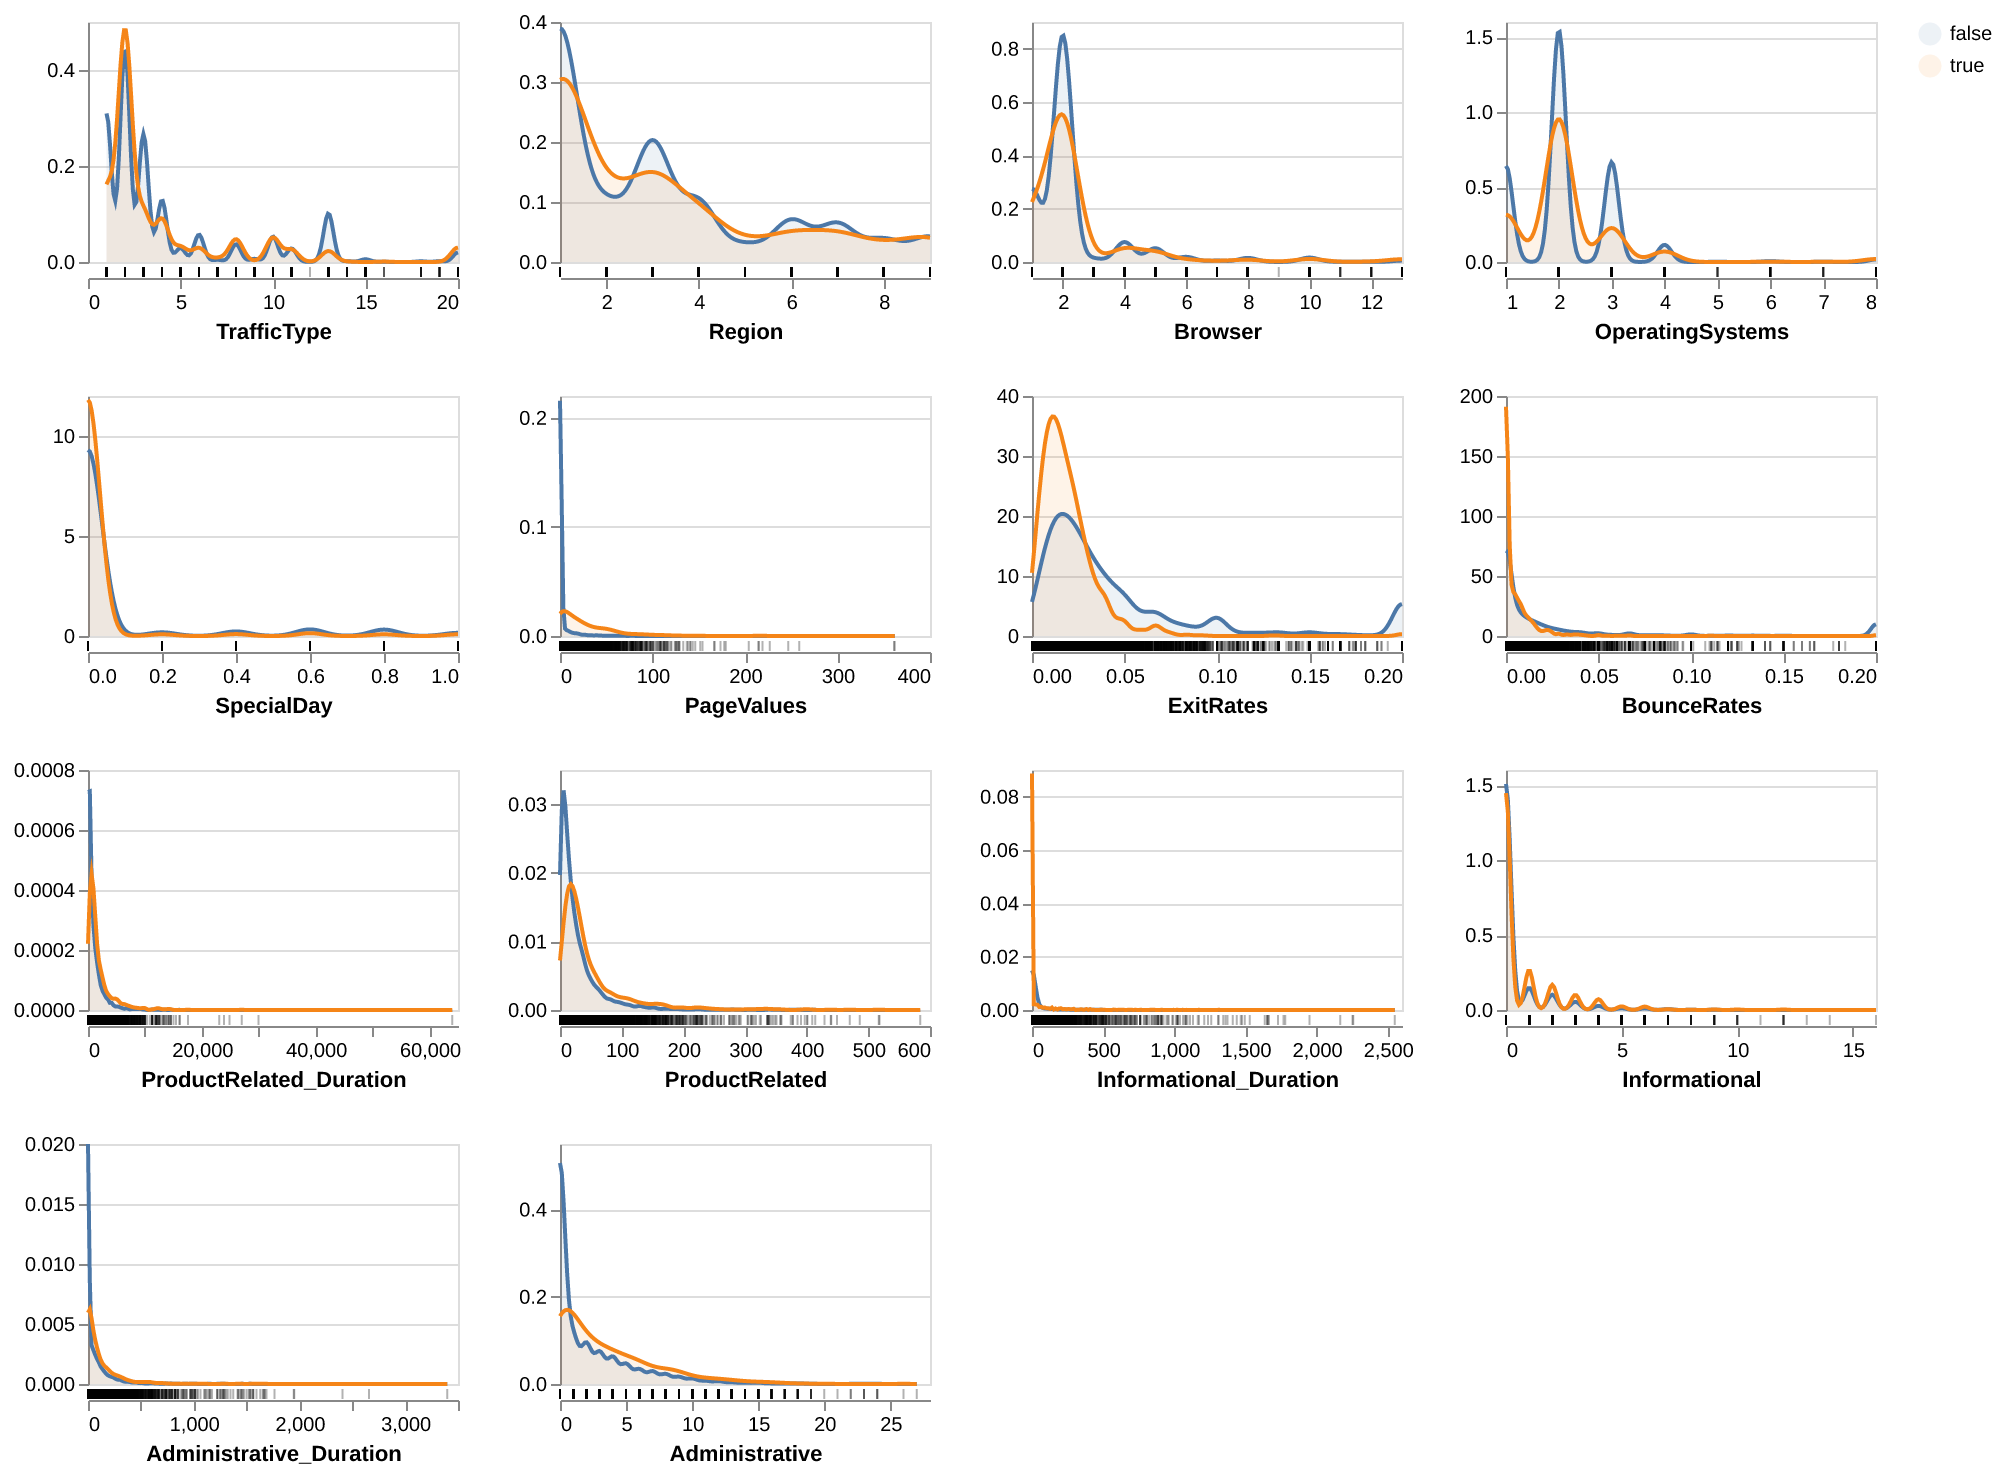
\includegraphics[width=0.65\textwidth,height=\textheight]{../results/images/feature_density.png}

}

\caption{\label{fig-feature_density}Distribution of numeric features for
each target class.}

\end{figure}%

\begin{figure}

\centering{

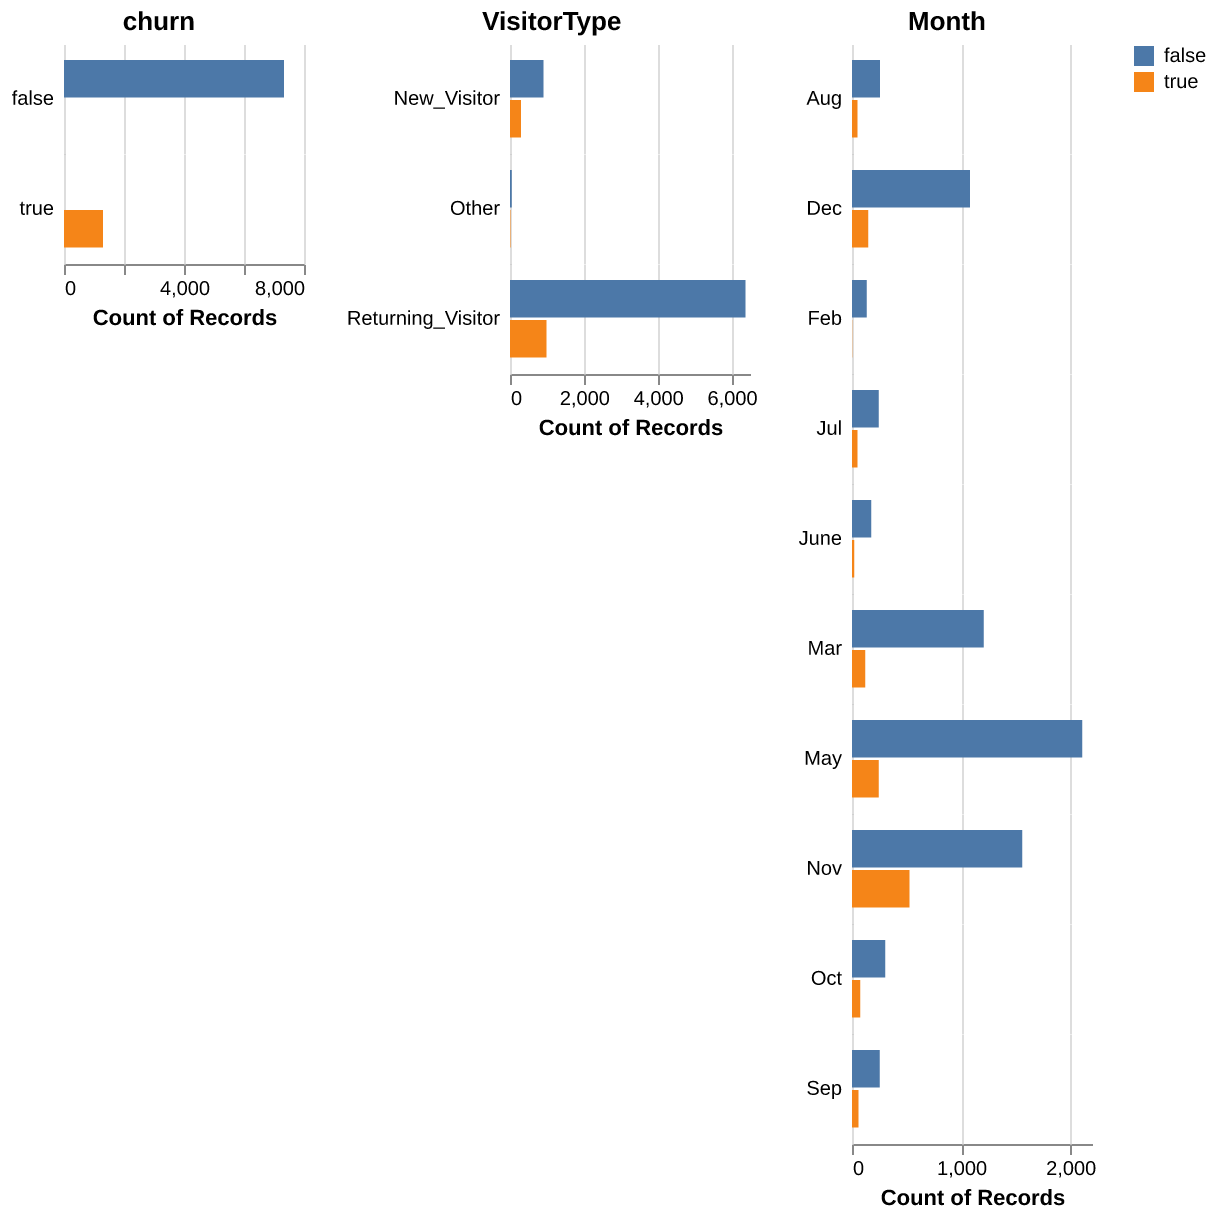
\includegraphics[width=0.65\textwidth,height=\textheight]{../results/images/feature_bar_plot.png}

}

\caption{\label{fig-feature_bar_plot}Distribution of categorical
features for each target class.}

\end{figure}%

\begin{figure}

\centering{

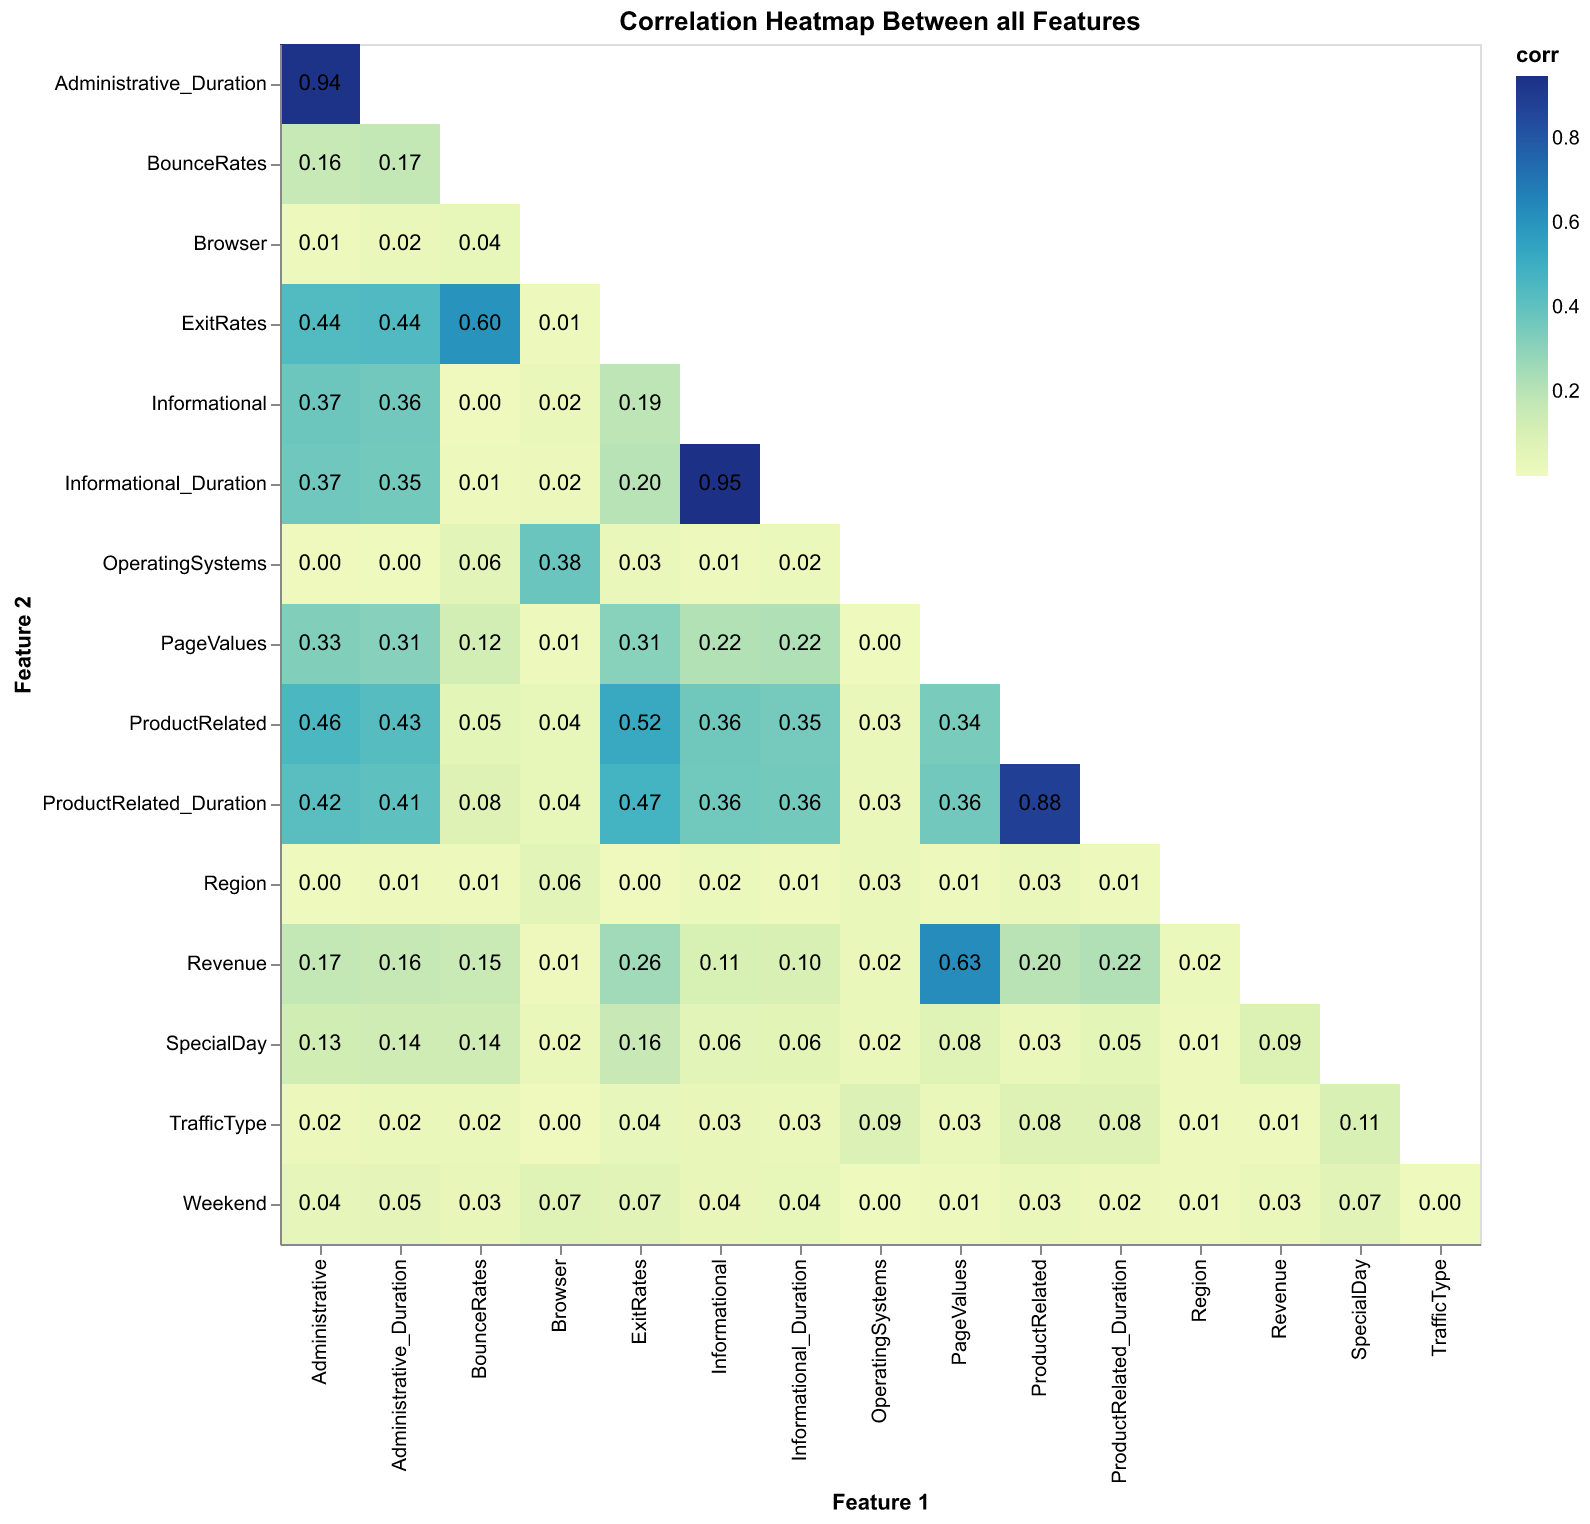
\includegraphics[width=0.65\textwidth,height=\textheight]{../results/images/correlation_heatmap.png}

}

\caption{\label{fig-correlation_heatmap}Correlation plot between all
features in dataset}

\end{figure}%

We chose to use a logistic regression model for our classification
model. To find the model with the highest acuracy in predicting our
target, we used 5-fold cross-validation to select our best value of the
C hyperparameter. We found that the best C was 0.768.

From cross-validation, we found that our best logistic regression model
with C = 0.768 yielded an validation accuracy score of 88.6\%, which is
slightly better (3.7\%) compared to the validation accuracy score of our
dummy classifier using a most-frequent strategy (84.9\%).

After testing our model using the testing data, we found that our best
logistic regression model with C = 0.768 had a test accuracy score of
87.6\%, which is again a bit better (4.1\%) that the test accuracy score
of our dummy classifier using a most-frequent strategy (83.5\%).

\begin{longtable}[]{@{}
  >{\raggedleft\arraybackslash}p{(\columnwidth - 8\tabcolsep) * \real{0.1569}}
  >{\raggedleft\arraybackslash}p{(\columnwidth - 8\tabcolsep) * \real{0.1373}}
  >{\raggedright\arraybackslash}p{(\columnwidth - 8\tabcolsep) * \real{0.2647}}
  >{\raggedleft\arraybackslash}p{(\columnwidth - 8\tabcolsep) * \real{0.2745}}
  >{\raggedleft\arraybackslash}p{(\columnwidth - 8\tabcolsep) * \real{0.1667}}@{}}

\caption{\label{tbl-dummy_bestmodel_scores}The comparison of scores
between Dummy Classifier and Logistic Regression model with the best
parameters.}

\tabularnewline

\toprule\noalign{}
\begin{minipage}[b]{\linewidth}\raggedleft
Unnamed: 0.1
\end{minipage} & \begin{minipage}[b]{\linewidth}\raggedleft
Unnamed: 0
\end{minipage} & \begin{minipage}[b]{\linewidth}\raggedright
model
\end{minipage} & \begin{minipage}[b]{\linewidth}\raggedleft
mean\_validation\_accuracy
\end{minipage} & \begin{minipage}[b]{\linewidth}\raggedleft
test\_accuracy
\end{minipage} \\
\midrule\noalign{}
\endhead
\bottomrule\noalign{}
\endlastfoot
0 & 0 & Dummy Model & 0.849496 & nan \\
1 & 1 & Logistic Regression Model & 0.886108 & nan \\

\end{longtable}

To find out how important each feature is considered by our model for
predicting the target class, we investigated the model's weight of each
feature in {[}@\#fig-feature\_bar\_plot{]}. We found that the
\texttt{ExitRates} and \texttt{PagesValues} features seem to be the most
important for determining the target.

\begin{figure}

\centering{

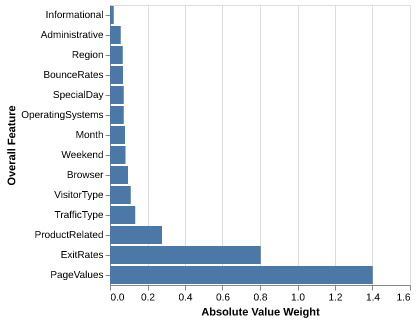
\includegraphics[width=0.65\textwidth,height=\textheight]{../results/images/fig4_feat_weights.png}

}

\caption{\label{fig-feature_bar_plot}Model features and their associated
absolute value weight.}

\end{figure}%

Our model achieves a high accuracy score of 87.6\%, suggesting its
potential usefulness in predicting whether a customer will purchase a
product based on their behavioral and interaction data with a business's
website. However, its performance is only marginally better than a model
that always predicts a customer will not make a purchase (accuracy =
83.5\%).

The analysis could be enhanced by addressing the imbalance in the target
classes within our data and by using alternative scoring metrics. This
approach might result in a better-performing model and a more robust
evaluation. Additionally, exploring other classification models, such as
SVM with RBF kernel and KNN, and comparing their performance to our
logistic regression model could provide valuable insights.

We also identified that the features \texttt{PageValue} (the average
value of web pages visited by the visitor) and \texttt{ExitRate} (the
average exit rate of web pages visited) were the most significant for
predictions. These findings offer meaningful insights into how
businesses can anticipate customer intentions and develop strategies to
increase sales, such as enhancing \texttt{PageValue} and reducing
\texttt{ExitRate} for potential customers. However, these insights may
evolve if the model incorporates the class imbalance in the data.

\subsection*{References}\label{references}
\addcontentsline{toc}{subsection}{References}

\phantomsection\label{refs}
\begin{CSLReferences}{1}{0}
\bibitem[\citeproctext]{ref-commerce2024ecommerce}
Commerce, Sellers. 2024. {``43 ECommerce Statistics in 2024 (Global and
u.s. Data).''} SellersCommerce.
\url{https://www.sellerscommerce.com/blog/ecommerce-statistics/}.

\bibitem[\citeproctext]{ref-numpy}
Harris, Charles R, K Jarrod Millman, Stéfan J van der Walt, Ralf
Gommers, Pauli Virtanen, David Cournapeau, Eric Wieser, et al. 2020.
{``{Array programming with NumPy}.''} \emph{Nature} 585 (7825): 357--62.
\url{https://doi.org/10.1038/s41586-020-2649-2}.

\bibitem[\citeproctext]{ref-pandas}
McKinney, Wes. 2010. {``Data Structures for Statistical Computing in
Python.''} In \emph{Proceedings of the 9th Python in Science
Conference}, edited by Stéfan van der Walt and Jarrod Millman, =51--56.

\bibitem[\citeproctext]{ref-scikit-learn}
Pedregosa, F., G. Varoquaux, A. Gramfort, V. Michel, B. Thirion, O.
Grisel, M. Blondel, et al. 2011. {``{Scikit-learn: Machine Learning in
Python}.''} \emph{Journal of Machine Learning Research} 12: 2825--30.

\bibitem[\citeproctext]{ref-sakar2018uci}
Sakar, C. O., S. O. Polat, M. Katircioglu, et al. 2018. {``UCI Machine
Learning Repository: Online Shoppers Purchasing Intention Dataset.''}
Neural Comput \& Applic.
\url{https://archive.ics.uci.edu/ml/datasets/Online+Shoppers+Purchasing+Intention+Dataset}.

\bibitem[\citeproctext]{ref-taheer2024online}
Taheer, Farrah. 2024. {``Online Shopping Statistics: How Many People
Shop Online in 2024?''} OptinMonster.
\url{https://optinmonster.com/online-shopping-statistics/}.

\bibitem[\citeproctext]{ref-truong2024ucimlrepo}
Truong, P. et al. 2024. {``Ucimlrepo Package.''} GitHub.
\url{https://github.com/uci-ml-repo/ucimlrepo/tree/main}.

\bibitem[\citeproctext]{ref-Python}
Van Rossum, Guido, and Fred L. Drake. 2009. \emph{Python 3 Reference
Manual}. Scotts Valley, CA: CreateSpace.

\bibitem[\citeproctext]{ref-altair}
VanderPlas, Jake. 2018. {``Altair: Interactive Statistical
Visualizations for Python.''} \emph{Journal of Open Source Software} 3
(7825, 32): 1057. \url{https://doi.org/10.21105/joss.01057}.

\end{CSLReferences}




\end{document}
